\documentclass[10pt,a4paper]{article}

\usepackage[T1]{fontenc}
\usepackage[utf8]{inputenc}
\usepackage{lmodern}
\usepackage[margin=2.4cm]{geometry}
\usepackage{amsmath,amssymb,amsthm}
\usepackage{booktabs}
\usepackage{tabularx}
\usepackage{graphicx}
\usepackage{xcolor}
\usepackage{algorithm}
\usepackage{algpseudocode}
\usepackage{pgfplots}
\pgfplotsset{compat=1.17}
\usepackage[numbers,sort&compress]{natbib}
\usepackage[hidelinks]{hyperref}

\definecolor{ramp300}{HTML}{6DA7EC}
\definecolor{ramp450}{HTML}{2A78D6}
\definecolor{ramp650}{HTML}{104281}
\definecolor{muted}{HTML}{6B6A64}

\newtheorem{proposition}{Proposition}
\newcommand{\Ms}{M_{\mathrm{s}}}
\newcommand{\Mmin}{M_{\min}}

\title{Hawking Cooling: Per-Searcher Step-Size Control from\\Black-Hole Evaporation, and a Controlled Test of Whether It Helps}
\author{Anton Erdmann Benz\\Bauhaus-Universit\"at Weimar\\\texttt{anton.erdmann.benz@uni-weimar.de}}
\date{October 2026}

\begin{document}
\maketitle

\begin{abstract}
Annealing-type optimisers usually lower a temperature by a schedule that is
global, prescribed in advance, and at most reset by an external trigger. We
describe a step-size rule in which each searcher in a population carries its own
temperature, derived from a mass that grows with the improvements it finds and
shrinks by Hawking evaporation while it stagnates. Because a black hole's
temperature is inversely proportional to its mass, the rule has negative heat
capacity: during consecutive failures a searcher heats up and its mass loss
accelerates until it is replaced by fresh searchers. Cooling, reheating and
restarts are therefore driven by each searcher's history, through a discrete
mass update and a fixed burst threshold, rather than by a global clock, and the
patience a searcher is granted grows with the improvement it has accumulated.
We derive continuous approximations to the temperature trajectory and survival
time in closed form, and test the rule in a controlled $2\times2$ factorial
design (reheating on or off, earned or fixed patience) against a fixed step size
and a per-searcher $1/5$ success rule, with shared proposal, selection and burst mechanics. On nine
problems (six synthetic functions in ten dimensions and three data-based tasks),
the Hawking rule beats a fixed step size on six problems, but its distinctive
ingredients provide no consistent benefit, and the $1/5$ control is significantly
better on eight of nine problems under unadjusted per-problem tests. We report
this negative result as the main finding, and identify a likely cause. Because
mass grows only in proportion to normalised improvement, each searcher's
temperature has a floor that does not shrink with the budget: in our runs the
Hawking step never fell below $0.016$ (in unit-cube units, about one-twelfth of
its initial value), whereas the $1/5$ step reached $10^{-3}$ or less on every
problem. Results for a larger algorithm built around the rule are given in an
appendix.
\end{abstract}

\section{Introduction}

Simulated annealing \citep{kirkpatrick1983,cerny1985} controls the balance between
exploration and exploitation with a temperature that is lowered over time. In most
variants the temperature is a single global quantity following a prescribed
schedule. Re-annealing \citep{ingber1989} rescales temperatures using search
sensitivities, while iterated local search and restart evolution strategies
\citep{lourenco2003,auger2005} perturb or reinitialise the search state. Parallel
tempering in its classical replica-exchange form \citep{hukushima1996} gives each replica its own
temperature, but those temperatures are fixed ladder rungs, not quantities each
replica earns.

This paper studies a different construction, taken from black-hole
thermodynamics. A Schwarzschild black hole of mass $M$ radiates at the Hawking
temperature $T \propto 1/M$ \citep{hawking1974,hawking1975} and loses mass at a
rate $\dot M \propto -1/M^2$ \citep{page1976}. Because its temperature rises as it
loses energy, it has negative heat capacity, a property shared with
self-gravitating systems \citep{lyndenbell1968,thirring1970}, and its evaporation
accelerates as mass decreases. We use this idealised mass-loss law as a search
analogy; the algorithm replaces the low-mass endpoint by an explicit restart.

We map this onto a population of searchers. Each searcher is a ``hole'' whose
mass grows when it finds improvements (accretion) and decays while it does not
(evaporation). Its mutation step length is its Hawking temperature $T = k/M$. The
resulting rule has three properties that, taken together, we have not found in the
step-size adaptation literature:
\begin{enumerate}
  \item \textbf{Per-searcher, unscheduled cooling.} Every searcher has its own
        temperature, driven by its own successes and failures. There is no global
        schedule or iteration-dependent decay.
  \item \textbf{Reheating with runaway.} Failure heats a searcher, and the heating
        accelerates; a stuck searcher drifts towards more and more exploratory steps
        before it is restarted.
  \item \textbf{Earned patience.} The number of consecutive failures a searcher
        survives grows approximately as a power of its post-success mass, so
        heavier searchers receive more time.
\end{enumerate}

Metaphor-based metaheuristics are rightly met with scepticism
\citep{sorensen2015,camacho2019}: a new vocabulary often disguises a known
mechanism. We therefore state the rule as plain update equations
(Section~\ref{sec:method}), derive its behaviour (Section~\ref{sec:analysis}), and
compare it against controls that switch off its distinctive ingredients one at a
time within a shared search loop (Sections~\ref{sec:setup}
and~\ref{sec:results}). The result is negative: in our setting the distinctive
ingredients provide no consistent benefit, and a fifty-year-old rule \citep{rechenberg1973} does
better. We think this is worth reporting, both to save others the effort and
because the failure has an identifiable cause: tying mass to accumulated
improvement puts a budget-independent floor under each searcher's temperature
(Proposition~\ref{prop:floor} and Section~\ref{sec:discussion}).

\section{Related work}
\label{sec:related}

\paragraph{Annealing and reheating.} Simulated annealing lowers a global temperature
on a fixed schedule \citep{kirkpatrick1983,cerny1985}. Very fast simulated
re-annealing \citep{ingber1989} periodically rescales per-parameter temperatures
using sensitivity estimates. Generalised simulated annealing
\citep{tsallis1996,xiang1997} supplies the visiting and acceptance framework used
by SciPy's hybrid \texttt{dual\_annealing} implementation \citep{virtanen2020}.
In that implementation, re-annealing is triggered when the scheduled temperature
reaches a specified fraction of its initial value \citep{scipydualannealingdocs}.
These mechanisms differ from a temperature coupled to each searcher's
accreting and evaporating mass.

\paragraph{Per-replica temperatures.} Replica Monte Carlo
\citep{swendsen1986} is an early multi-temperature approach. In classical
replica exchange \citep{hukushima1996}, configurations are exchanged between
slots with fixed temperatures. Temperature belongs to the slot rather than
being earned or lost by a configuration.

\paragraph{Step-size adaptation in evolution strategies.} The $1/5$ success rule
\citep{rechenberg1973,schwefel1981} increases the step length when the measured
success frequency exceeds $1/5$ and reduces it when it falls below that target.
The classical formulation measures success over blocks of trials
\citep{beyer2002}; our controls use a per-trial multiplicative variant.
Self-adaptation and cumulative step-size adaptation, as in CMA-ES
\citep{hansen2001,beyer2002}, provide other mechanisms for adapting mutation scale
and shape. The Hawking rule moves the step size
in the \emph{opposite} direction: success shrinks it and failure enlarges it.

\paragraph{Escalation and abandonment.} Basic variable neighbourhood search
\citep{mladenovic1997} advances through a predefined sequence of neighbourhoods
after failure and returns to the first after improvement; the neighbourhoods
need not be nested. The artificial bee colony algorithm \citep{karaboga2007}
uses a common fixed limit without improvement to trigger food-source abandonment.
Iterated local search \citep{lourenco2003} combines
local optimisation with perturbation and acceptance decisions, which can depend
on search history. Restart CMA-ES \citep{auger2005} reinitialises the search
distribution and increases the population size across restarts. These methods
provide broader precedents for escaping stagnation than a single fixed failure limit.

\paragraph{Black-hole metaheuristics.} The original Black Hole algorithm
\citep{hatamlou2013} treats the best solution as an attractor and replaces
candidates that cross its event horizon with random ones. Its variants are
reviewed by \citet{abualigah2022}. Nemati and Momeni's fuzzy black-holes algorithm
uses ``Hawking radiation'' for positional mutation with a fitness-dependent
mutation probability \citep{nemati2014}, rather than the evaporating-mass
proposal scale studied here. Related physics-inspired methods use gravitational attraction between
fitness-weighted masses \citep{rashedi2009} or black-, white- and wormhole transfer
between candidate universes \citep{mirjalili2016}. This comparison concerns the
mechanisms in the cited works; it is not a systematic novelty search and does
not establish a comprehensive priority claim.

\section{Method}
\label{sec:method}

We consider minimisation. The search runs in the unit cube $[0,1]^d$, mapped affinely onto the problem's box,
so that step lengths are comparable across problems. Each searcher $i$ holds a
position $x_i$, its objective value $f_i$, a mass $M_i$ and a starvation counter
$n_i$ (iterations since its last success). Let $s$ be the standard deviation of the
objective over the initial population, held fixed throughout the run to make mass gain unit-free; if it is zero, we use
$s=1$. Here ``temperature'' means mutation scale, not an acceptance temperature:
only strictly improving proposals are accepted.

\paragraph{Temperature and moves.} The temperature of searcher $i$ is
\begin{equation}
  T_i = k / M_i, \label{eq:temperature}
\end{equation}
and it proposes $x' = \operatorname{reflect}\!\left(x_i + (T_i/\sqrt d)\,z\right)$
with $z\sim\mathcal N(0,I_d)$, where $\operatorname{reflect}$ mirrors points back into
the cube. Before reflection, the factor $1/\sqrt d$ gives
$\mathbb E\lVert (T_i/\sqrt d)z\rVert^2=T_i^2$: $T_i$ is the root-mean-square proposal
length, not its expected Euclidean length. Reflection changes the realised length.

\paragraph{Accretion.} If $f(x') < f_i$, the searcher moves and gains mass in
proportion to the improvement:
\begin{equation}
  M_i \leftarrow M_i + \min\!\left(g\,\frac{f_i - f(x')}{s},\; M_i\right),\qquad n_i \leftarrow 0.
  \label{eq:accretion}
\end{equation}
The cap stops one lucky step from more than doubling the mass. The implementation
also caps the resulting mass at $M_{\max}=10^5$. The position and stored objective
value are then updated to $x'$ and $f(x')$.

\paragraph{Evaporation.} Otherwise the searcher stays put and evaporates by a
discretised $\dot M = -\alpha/M^2$, with a time step equal to its starvation counter:
\begin{equation}
  n_i \leftarrow n_i + 1,\qquad M_i \leftarrow M_i - \alpha\,n_i / M_i^2.
  \label{eq:evaporation}
\end{equation}
Success causes no evaporation and resets $n_i$. Weighting a failed update by
$n_i$ rather than $1$ further accelerates mass loss during a failure streak. This
starvation weighting is an algorithmic addition to the Hawking mass-loss law. Section~\ref{sec:results} also tests the plain version with time step $1$.

\paragraph{Final burst.} When $M_i < \Mmin$, the searcher is replaced by a child at
$\operatorname{reflect}(x_i + (k/\Mmin)/\sqrt d\,z)$ with mass $m_c$, and up to $b-1$
further children are added while the population is below a cap of $2N$. In the
implementation, replacement happens immediately: additional children are centred
on the first child rather than the old parent. Each child is evaluated and its
starvation counter starts at zero; additional children enter the next population
sweep. The best evaluated point is retained separately, even if its searcher bursts.

Algorithm~\ref{alg:hawking} gives the complete loop. Table~\ref{tab:params} in Appendix~\ref{app:repro} lists the mass, step-size and
population parameters. Every objective call, including initialisation and burst
children, counts against the budget; the run stops immediately when it is exhausted.

\begin{algorithm}[t]
\caption{Hawking cooling for a population of $N$ searchers.}
\label{alg:hawking}
\begin{algorithmic}[1]
\State initialise $x_i \sim U[0,1]^d$, $f_i \gets f(x_i)$, $M_i \gets M_0$, $n_i \gets 0$ for $i=1..N$
\State $s \gets \operatorname{std}_i f_i$ (use $1$ if zero); retain the best evaluated point
\While{budget remains}
  \ForAll{searchers $i$ present at the start of this sweep}
    \State draw $z\sim\mathcal N(0,I_d)$; $T_i \gets k/M_i$; $x' \gets \operatorname{reflect}(x_i + (T_i/\sqrt d)\,z)$
    \State $f' \gets f(x')$; update the best evaluated point
    \If{$f' < f_i$}
      \State $M_i \gets \min\{M_{\max}, M_i + \min(g\,(f_i-f')/s,\,M_i)\}$
      \State $x_i \gets x'$; $f_i \gets f'$; $n_i \gets 0$ \Comment{accretion: cools}
    \Else
      \State $n_i \gets n_i + 1$; \quad $M_i \gets M_i - \alpha\, n_i / M_i^2$ \Comment{evaporation: heats}
    \EndIf
    \If{$M_i < \Mmin$}
      \State evaluate a replacement child at scale $k/\Mmin$; set its mass to $m_c$, counter to $0$
      \State evaluate up to $b-1$ extra children around that child, subject to the cap $2N$
      \State retain the best evaluated point; queue extra children for the next sweep
    \EndIf
  \EndFor
\EndWhile
\State \Return best evaluated point
\end{algorithmic}
\end{algorithm}

\section{Analysis}
\label{sec:analysis}

Consider a searcher whose last success left it with mass $\Ms$, and treat the
failure count $n$ as continuous.

\begin{proposition}[Negative heat capacity]
Under~\eqref{eq:temperature}, $C = dM/dT = -k/T^2 = -M^2/k < 0$. Mass loss raises the
temperature, and mass gain lowers it.
\end{proposition}

\begin{proposition}[Continuous temperature trajectory and survival time]
Approximate the discrete failure updates by $dM/dn=-\alpha n/M^2$, starting from
$M(0)=\Ms>\Mmin$. Then $M(n)^3=\Ms^3-\tfrac32\alpha n^2$, and
\begin{equation}
  T(n) = k\left(\Ms^3 - \tfrac32 \alpha n^2\right)^{-1/3},\qquad
  n^\ast = \sqrt{\frac{2\,(\Ms^3 - \Mmin^3)}{3\alpha}}.
  \label{eq:survival}
\end{equation}
Here $n^\ast$ is the continuous threshold-crossing time; it scales as
$\Ms^{3/2}$ when $\Ms\gg\Mmin$. For the unit-step approximation
$dM/dn=-\alpha/M^2$, the corresponding time is
$n^\ast=(\Ms^3-\Mmin^3)/(3\alpha)$, scaling as $\Ms^3$.
\end{proposition}
\begin{proof}
Multiplying the first differential equation by $3M^2$ gives
$d(M^3)/dn=-3\alpha n$. Integrating and solving $M(n^\ast)=\Mmin$ gives the
result. The unit-step case instead has $d(M^3)/dn=-3\alpha$.
\end{proof}

These expressions are not exact solutions of the implemented Euler update.
For its $j$th consecutive failure, cubing~\eqref{eq:evaporation} gives
\begin{equation}
 M_j^3=M_{j-1}^3-3\alpha j
       +\frac{3\alpha^2j^2}{M_{j-1}^3}
       -\frac{\alpha^3j^3}{M_{j-1}^6}.
 \label{eq:discrete-mass}
\end{equation}
Dropping the higher-order terms yields
$M_n^3\approx\Ms^3-\tfrac32\alpha n(n+1)$. This approximation requires small
relative decrements $\alpha j/M_{j-1}^3$ and can fail near the burst threshold.
The actual burst occurs at the first integer $j$ for which $M_j<\Mmin$.

\begin{proposition}[Runaway]
In the continuous approximation, $dT/dn = \alpha n\,T^4/k^3$, which increases in both $n$ and $T$. A failing searcher
heats slowly at first and then ever faster, up to the burst temperature $k/\Mmin$.
\end{proposition}
\begin{proof}
$dT/dn = -(k/M^2)\,dM/dn = k\alpha n / M^4 = \alpha n\, T^4/k^3$.
\end{proof}

Figure~\ref{fig:trajectory} plots~\eqref{eq:survival} for the default parameters. A
searcher with $\Ms = 1$ reaches the continuous threshold at about 8 failures;
one with $\Ms = 10$ reaches it at about 258. These are illustrative values for
$\alpha=0.01$, not the tuned value $0.001$ used for Hawking in the main comparison. The temperature stays near its post-success
value for most of that time and rises steeply only at the end.

A final property limits how cold a searcher can become.

\begin{proposition}[Temperature floor]
\label{prop:floor}
Let a searcher be created with mass $m$ (either $M_0$ or $m_c$) at a point with
objective value $f_{\mathrm b}$, and let $f^\ast$ be the minimum of the
objective over the box. At every iteration of its lifetime,
\begin{equation}
  M_i \le m + g\,\frac{f_{\mathrm b}-f^\ast}{s},\qquad
  T_i \ge \frac{k}{m + g\,(f_{\mathrm b}-f^\ast)/s}.
  \label{eq:floor}
\end{equation}
\end{proposition}
\begin{proof}
Evaporation and the ceiling $M_{\max}$ only reduce mass, and a success from
$f_i$ to $f'$ adds at most $g\,(f_i-f')/s$. Because the stored value $f_i$ only
decreases, these increments telescope to at most
$g\,(f_{\mathrm b}-f_i)/s\le g\,(f_{\mathrm b}-f^\ast)/s$.
\end{proof}

The bound depends on the starting point and on the initial spread $s$, but not
on the budget or on the number of successes. For a random start,
$(f_{\mathrm b}-f^\ast)/s$ is typically a few units, so with $g=2$ the
temperature cannot fall much more than an order of magnitude below $k/M_0$. The
no-reheating variants of Section~\ref{sec:setup} share the accretion law and
hence the floor. Section~\ref{sec:discussion} reports the scales reached in
practice.

\begin{figure}[t]
\centering
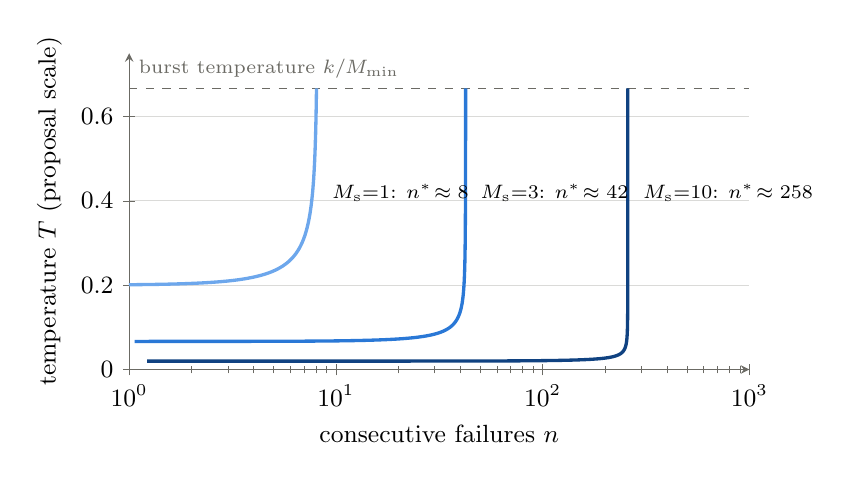
\begin{tikzpicture}
\begin{axis}[
  width=0.78\linewidth, height=5.6cm,
  xmode=log, xmin=1, xmax=1000,
  ymin=0, ymax=0.75,
  xlabel={consecutive failures $n$},
  ylabel={temperature $T$ (proposal scale)},
  axis lines=left, tick style={muted}, axis line style={muted},
  label style={font=\small}, tick label style={font=\small},
  ymajorgrids, grid style={muted!25},
  clip=false,
]
\addplot[muted, dashed, thin, domain=1:1000] {0.2/0.3};
\node[font=\scriptsize, text=muted, anchor=south west] at (axis cs:1,0.667) {burst temperature $k/M_{\min}$};
% parametric in the mass M: n(M) = sqrt((Ms^3 - M^3) / (1.5 alpha)), T = k/M
\addplot[ramp300, line width=1.2pt, domain=0.3:0.995, samples=200, variable=\m] ({sqrt((1-\m^3)/0.015)}, {0.2/\m});
\addplot[ramp450, line width=1.2pt, domain=0.3:2.9994, samples=300, variable=\m] ({sqrt((27-\m^3)/0.015)}, {0.2/\m});
\addplot[ramp650, line width=1.2pt, domain=0.3:9.99995, samples=400, variable=\m] ({sqrt((1000-\m^3)/0.015)}, {0.2/\m});
\node[font=\scriptsize, anchor=west] at (axis cs:8.6,0.42) {$M_{\mathrm s}{=}1$: $n^\ast\!\approx 8$};
\node[font=\scriptsize, anchor=west] at (axis cs:45,0.42) {$M_{\mathrm s}{=}3$: $n^\ast\!\approx 42$};
\node[font=\scriptsize, anchor=west] at (axis cs:275,0.42) {$M_{\mathrm s}{=}10$: $n^\ast\!\approx 258$};
\end{axis}
\end{tikzpicture}
\caption{Temperature of a stagnating searcher after its last success at mass
$M_{\mathrm s}$, from~\eqref{eq:survival} with $k=0.2$, $\alpha=0.01$, $M_{\min}=0.3$. Each
curve ends at the continuous burst threshold. Heavier searchers stay cold longer; the threshold time scales as
$M_{\mathrm s}^{3/2}$ for masses well above $M_{\min}$.}
\label{fig:trajectory}
\end{figure}

\section{Experimental setup}
\label{sec:setup}

\paragraph{Problems.} Nine minimisation problems: sphere, Rosenbrock, Rastrigin,
Ackley, Griewank and Schwefel in $d=10$; maximum elevation on a $30$\,m digital
elevation model of the Jacksboro Fault, Tennessee ($d=2$, error in metres); and
$k$-means clustering of the Iris ($d=12$) and Wine ($d=39$) data sets, with reference
values taken from the best of 50 $k$-means++ restarts with random seed zero.
For clustering, features are standardised to zero mean and unit variance, and the
objective is the mean squared distance to the nearest of three centres. These
reference values are empirical, not certified global optima. We report
$e=\max(f-f^{\mathrm{ref}},0)$, using known optima for the synthetic functions and
the highest grid elevation for terrain. Clipping prevents negative errors from
roundoff or a better-than-reference solution; zero does not certify optimality.

\paragraph{Controls.} All variants share the loop of Algorithm~\ref{alg:hawking}:
population $N=20$, Gaussian proposal standard deviation $T/\sqrt d$ per coordinate, reflection,
and a three-child burst at temperature $k/\Mmin$ with a population cap of 40. Mergers
and all other modules of the larger algorithm (Appendix~\ref{app:full}) are switched
off, so the variants differ only in how a searcher sets its step length and when it
gives up:
\begin{itemize}
  \item \textbf{Hawking}: the rule of Section~\ref{sec:method} (reheating, earned patience).
  \item \textbf{Hawking, $\Delta t=1$}: evaporation with a unit time step (survival $\propto \Ms^3$).
  \item \textbf{No reheating, earned patience}: the same mass-based burst criterion as Hawking, but
        the step length stays at $k/\Ms$, the value set by the last success.
  \item \textbf{Reheating, fixed patience}: Hawking temperature, saturating at $k/\Mmin$,
        but the burst comes after $L$ consecutive failures.
  \item \textbf{No reheating, fixed patience}: step length $k/\Ms$; burst after $L$ failures.
  \item \textbf{$1/5$ rule, fixed patience}: per-searcher step $\sigma$, multiplied by
        $1.5$ on success (capped at $1$) and by $1.5^{-1/4}$ on failure. This is a
        per-trial controller inspired by the $1/5$ success rule
        \citep{rechenberg1973,beyer2002}; burst after $L$ failures, analogous to
        the fixed abandonment limit in artificial bee colony \citep{karaboga2007}.
  \item \textbf{$1/5$ rule, earned patience}: the $1/5$ step rule, with burst timing
        from the evaporating mass as in Hawking.
  \item \textbf{Fixed step}: step $k/M_0$ for initial searchers and $k/m_c$ for
        burst children, constant within each lifetime; burst after $L$ failures.
\end{itemize}
Hawking, no reheating with earned patience, reheating with fixed patience, and
no reheating with fixed patience form the $2\times2$ design. Each is tuned
separately. The contrasts compare complete tuned variants, rather than isolating
a change at a common parameter setting or estimating a formal factorial effect.
In the no-reheating, fixed-patience cell, mass is not evaporated; it only increases
on success and resets at a burst. Thus this cell also changes the mass from which
subsequent success-driven cooling proceeds.

\paragraph{Protocol.} Each run has a budget of $10\,000$ objective evaluations counted by
a shared wrapper. Every variant gets one tuned parameter, chosen by mean rank on
screening seeds 100--104 from a four-value grid: $L \in \{8, 30, 100, 300\}$ for
fixed patience, and $\alpha \in \{0.001, 0.003, 0.01, 0.03\}$ for earned patience. The
reported comparison uses 15 different seeds (0--14). Differences are tested per problem
with a two-sided Mann--Whitney $U$ test \citep{mannwhitney1947} at $p<0.05$, without
correction for multiple comparisons. We treat these as exploratory comparisons,
not tests of equivalence. The test compares distributions rather than medians
alone; win/loss labels use the direction of the observed median difference.
Mean rank is the average, across problems, of ranks of
the unrounded median errors; exact ties are ordered by the fixed variant order
in the analysis script. Appendix~\ref{app:repro} describes the implementation and
reproducibility materials.

\section{Results}
\label{sec:results}

\begin{table}[t]
\centering
\footnotesize
\setlength{\tabcolsep}{3.4pt}
\caption{Median final error over 15 seeds ($10\,000$ evaluations). Lower is better;
\textbf{bold} marks the best median per problem and the best mean rank. The last column counts problems on
which Hawking is significantly better / no difference is detected / significantly worse
(Mann--Whitney $U$, $p<0.05$).}
\label{tab:controls}
\begin{tabular}{@{}llrrrrrrrrrcc@{}}
\toprule
variant & tuned & sph & rosen & rastr & ackley & griew & schwef & terrain & iris & wine & rank & W/T/L \\
\midrule
Hawking                     & $\alpha$=.001 & 7.6e-3 & 23.2 & 37.8 & 17.8 & 0.878 & 1170 & 4.17 & 1.9e-3 & 2.98 & 5.56 & -- \\
Hawking, $\Delta t=1$       & $\alpha$=.01  & 8.5e-3 & 21.6 & 42.8 & 18.0 & 0.880 & 1170 & 2.68 & 1.6e-3 & 2.91 & 5.11 & 0/8/1 \\
no reheat, earned           & $\alpha$=.003 & 9.3e-3 & 23.5 & 36.2 & 16.9 & 0.871 & 1100 & 3.42 & 2.0e-3 & 2.97 & 5.00 & 1/8/0 \\
reheat, fixed $L$           & $L$=100       & 1.1e-2 & 37.2 & 33.9 & 13.5 & 0.874 & 1060 & 3.45 & 2.2e-3 & 2.82 & 4.78 & 1/7/1 \\
no reheat, fixed $L$        & $L$=100       & 1.2e-2 & 19.4 & 38.6 & 16.4 & 0.899 & 1070 & 3.76 & 2.0e-3 & 2.99 & 5.67 & 0/8/1 \\
\midrule
$1/5$ rule, fixed $L$       & $L$=100       & \textbf{3.4e-7} & \textbf{3.03} & \textbf{27.9} & \textbf{1.65} & \textbf{0.040} & \textbf{1050} & \textbf{8.8e-9} & \textbf{4.2e-6} & \textbf{2.08} & 1.56 & 0/1/8 \\
$1/5$ rule, earned          & $\alpha$=.001 & \textbf{3.4e-7} & 3.34 & \textbf{27.9} & 2.04 & \textbf{0.040} & \textbf{1050} & 4.4e-7 & 4.3e-6 & \textbf{2.08} & \textbf{1.44} & 0/1/8 \\
fixed step                  & $L$=300       & 0.479 & 134 & 50.6 & 7.20 & 2.64 & 1580 & 5.95 & 3.5e-2 & 2.32 & 6.89 & 6/1/2 \\
\bottomrule
\end{tabular}
\end{table}

Table~\ref{tab:controls} gives the results. We draw four conclusions.

\paragraph{The adaptive rule improves on the fixed-step control.} Hawking has
significantly lower error on six problems and higher error on two (Ackley and
Wine). This supports the combined adaptive rule relative to this particular
fixed-step baseline; it does not isolate the mass--temperature coupling from
its restart criterion.

\paragraph{Reheating provides no consistent benefit.} With earned patience,
Hawking improves significantly on the no-reheating variant only on sphere.
With fixed patience, reheating is significantly worse on Rosenbrock and better
on Ackley. The mean ranks of the four factorial cells range from 4.78 to 5.67.
These mixed results do not establish that reheating has no effect.

\paragraph{Earned patience provides no consistent benefit.} With reheating,
earned patience is significantly better on sphere and worse on Ackley than the
fixed limit. Without reheating, it is significantly worse on Rosenbrock, with
no detected difference on the other eight problems. With the $1/5$ step rule,
no difference between earned and fixed patience is detected on any problem.
The unit-step Hawking variant is significantly better than the starvation-clock
variant only on terrain. A non-significant comparison does not establish
performance equivalence.

\paragraph{The $1/5$ controls perform best.} Both $1/5$ variants have significantly
lower error than Hawking on eight of nine problems, with no detected difference
on Schwefel. Several differences span orders of magnitude (sphere:
$3\times10^{-7}$ versus $8\times10^{-3}$; terrain: $10^{-8}$ versus $4$\,m for
fixed patience). These conclusions use the unadjusted tests specified above.

\section{Discussion}
\label{sec:discussion}

\begin{table}[t]
\centering
\footnotesize
\setlength{\tabcolsep}{3.4pt}
\caption{Smallest proposal scale (unit-cube RMS step) used by any searcher in a
run, median over seeds 0--14 at the selected settings of
Table~\ref{tab:controls}. The initial scale is $k/M_0=0.2$.}
\label{tab:floor}
\begin{tabular}{@{}lrrrrrrrrr@{}}
\toprule
variant & sph & rosen & rastr & ackley & griew & schwef & terrain & iris & wine \\
\midrule
Hawking               & 0.016 & 0.023 & 0.023 & 0.017 & 0.016 & 0.017 & 0.023 & 0.018 & 0.017 \\
no reheat, earned     & 0.016 & 0.023 & 0.023 & 0.017 & 0.016 & 0.017 & 0.022 & 0.018 & 0.017 \\
$1/5$ rule, fixed $L$ & 2.2e-5 & 1.2e-4 & 3.5e-6 & 4.6e-7 & 8.8e-6 & 9.8e-9 & 7.3e-16 & 3.3e-5 & 9.3e-4 \\
\bottomrule
\end{tabular}
\end{table}

\paragraph{A likely cause of the performance gap: the temperature floor.}
Proposition~\ref{prop:floor} bounds each searcher's temperature from below by a
quantity that does not depend on the budget, and Table~\ref{tab:floor} shows
that the bound is reached in practice. On every problem, neither Hawking nor
its no-reheating counterpart ever proposed a step smaller than $0.016$, about
one-twelfth of the initial scale. The $1/5$ controller changes its scale by a
fixed factor per trial, whatever the size of the improvement, and reached
$10^{-3}$ or less on all nine problems. Near the minimum of a smooth function,
sustained progress requires a step that shrinks in proportion to the distance
to the optimum \citep{rechenberg1973,beyer2002}. Once that distance falls well
below the floor, success becomes rare, and the searcher evaporates and bursts
instead of refining. This is consistent with where the gaps in
Table~\ref{tab:controls} are largest: on sphere, terrain and Iris, the $1/5$
controls reach errors between two and eight orders of magnitude lower. On
Rastrigin, Schwefel and Wine, where final precision matters less than which
basin is found, the medians differ by less than a factor of $1.5$. Because
the no-reheating variants share the floor, it also explains why switching
reheating off does not help. The diagnostic shows that the floor binds. It
does not prove that the floor causes the gap, which would require an
intervention that removes it.

\paragraph{Feedback direction.} A second difference is the sign of the feedback.
Each Hawking success adds mass and reduces the next proposal scale, whereas the
$1/5$ controller increases its scale on success and reduces it on failure. On
model problems such as the sphere, progress-rate analysis shows that this keeps
the success probability near a useful target \citep{rechenberg1973,beyer2002}.
Under the Hawking rule, both directions are self-reinforcing: smaller steps tend
to succeed more often and so cool further, while larger steps fail more often
and so heat further. The floor caps the first effect and the burst ends the
second. We have not separated the contributions of the floor and the feedback
direction. Terrain and clustering objectives are only piecewise smooth, so
smooth-model theory does not directly cover them.

\paragraph{What survives.} The equations do produce the intended qualitative behaviour:
unscheduled per-searcher cooling and reheating, and patience that grows with
accumulated improvement (Figure~\ref{fig:trajectory}). Mass links proposal scale and restart patience, although the implemented rule
still requires both a starvation counter and a burst threshold. We found
no performance benefit from that behaviour here. A version that keeps the
evaporation clock only as a restart criterion, and lets a $1/5$ rule set the step
(``$1/5$ rule, earned''), has no detected performance difference from the fixed-patience control and needs no tuned
abandonment limit $L$, though it needs a tuned $\alpha$ instead.

\paragraph{Limitations.} We tested one dimension for the synthetic problems ($d=10$),
one budget, nine problems and 15 seeds. Grids had four values per variant, and the
screening seeds used the same problems as the evaluation. Significance tests were not
corrected for multiplicity, and lack of significance is not evidence of equivalence.
Shared seed labels do not make the variants follow matched trajectories; the
reported Mann--Whitney tests compare their run distributions without using pairing.
The temperature-floor diagnostic (Table~\ref{tab:floor}) measures the scales
reached; it does not test an intervention. The larger algorithm in Appendix~\ref{app:full} was
developed on the same nine problems. The literature comparison in
Section~\ref{sec:related} is not a systematic review.

\section{Conclusion}

We formalised a step-size rule in which each searcher's temperature is the Hawking
temperature of an accreting and evaporating mass, derived continuous approximations to its trajectory and
$\Ms^{3/2}$ survival scaling, and tested its distinctive ingredients in a controlled design.
The combined rule outperforms the fixed-step control on six problems, but its reheating and earned
patience showed no consistent benefit, and the per-trial $1/5$ controller was
significantly better on eight of nine problems under exploratory, unadjusted tests.
The analogy produces the intended dynamics, but tying mass to accumulated
improvement puts a floor under the temperature that limits fine convergence.
Removing that floor, for instance with multiplicative accretion, is the natural
next test. Such a rule moves towards an inverted success-rule controller,
however, and any advantage over the $1/5$ rule would have to be shown rather
than assumed. Using mass only to time restarts looks less promising: our $1/5$
control with earned patience already does this and shows no detected advantage
over tuned fixed patience.

\bibliographystyle{plainnat}
\bibliography{refs}

\appendix

\section{Implementation details and reproducibility}
\label{app:repro}

\subsection{Scope of the implementation}

The experiments use \emph{Hawking search}, a Python software project containing
objective functions, a shared evaluation-budget wrapper, the controlled
variants, an extended population optimiser, and baseline implementations. The
associated project address is
\url{https://github.com/benzae1/hawkingsearch}. The mathematical method and
experimental protocol are specified here so that the paper can be read without
navigating the source tree. The companion software documentation provides the
installation steps, commands, and mapping from experiments to saved data.

There are three distinct configurations. The main study uses the core rule
with \emph{no mergers} and the parameters in Table~\ref{tab:params}. The
\emph{minimal implementation} additionally merges overlapping searchers and is
included only in the exploratory comparison in Appendix~\ref{app:full}. The
\emph{extended optimiser} adds population interactions and local refinement,
uses separately tuned settings, and is not a controlled test of the cooling
rule. The term ``Hawking'' in Table~\ref{tab:controls} refers only to the first
configuration.

\subsection{Core settings and control conventions}

\begin{table}[htbp]
\centering
\small
\caption{Core-rule settings for the controlled experiment. $\alpha$ is tuned for
earned-patience variants; fixed-patience variants tune $L$. These settings differ
from those of the extended optimiser in Appendix~\ref{app:full}.}
\label{tab:params}
\begin{tabular}{@{}llr@{}}
\toprule
symbol & meaning & value \\
\midrule
$N$       & initial population (cap $2N$)          & 20 \\
$M_0$     & initial mass                           & 1.0 \\
$k$       & temperature constant, $T = k/M$         & 0.2 \\
$g$       & accretion gain                         & 2.0 \\
$\alpha$  & evaporation constant                   & 0.01 (default) \\
$\Mmin$   & burst threshold                        & 0.3 \\
$m_c$     & mass of burst children                 & 0.6 \\
$b$       & maximum children per burst             & 3 \\
$M_{\max}$ & numerical mass ceiling                & $10^5$ \\
\bottomrule
\end{tabular}
\end{table}

For controls that retain an evaporating mass, its numerical ceiling is the
same as in the core rule. The no-reheating controls hold the proposal scale at
$k/M_{\mathrm s}$ between successes, where $M_{\mathrm s}$ is refreshed from the
current mass after each successful update. The reheating, fixed-patience
control uses $\alpha=0.01$ and clips mass below at $\Mmin$; its restart is
triggered only by $L$. The $1/5$ controls initialise their scale at $k/M_0$,
reset it to $k/m_c$ for burst children, cap it at $1$ after success, and impose
no lower scale bound. The fixed-step control likewise resets burst children
to $k/m_c$: its scale is constant over a searcher's lifetime, rather than
identical for initial searchers and their descendants. All controls share the
burst procedure and evaluation accounting described in Section~\ref{sec:method}.

Away from the upper cap, a success probability $p$ gives expected log-scale
change $\log(1.5)\,[p-(1-p)/4]$, which is zero at $p=1/5$. This explains the
target of the chosen per-trial multipliers; the values and cap are experimental
settings, not constants prescribed by the original $1/5$ rule.

\subsection{Data and numerical reproducibility}

The controlled study stores one record per variant, parameter setting, problem
and seed, including screening and evaluation runs. Its summary uses only seeds
0--14 at each variant's selected setting. Before running the study, the script
checks equality of the controlled Hawking implementation with the minimal
implementation when mergers are enabled, on Rastrigin with seed 3 and a budget
of 2\,000 evaluations. This is a regression check on one case, not a proof of
implementation equivalence for all inputs. The temperature-floor diagnostic in
Table~\ref{tab:floor} reruns the selected Hawking, no-reheating (earned) and
$1/5$ (fixed) settings on seeds 0--14 and records the smallest proposal scale
used by any searcher in each run.

The terrain data are the Jacksboro Fault elevation sample bundled with
Matplotlib; Iris and Wine are the bundled scikit-learn data sets. No network
data download is needed for these tasks. Numerical results can depend on
library versions and floating-point arithmetic, particularly near machine
precision and when a run can terminate in different local basins. A zero in a
result table means zero clipped error against the stated reference, not a
certified global optimum.

\section{Exploratory results for the extended optimiser}
\label{app:full}

\subsection{Purpose and additional mechanisms}

This appendix asks whether a larger optimiser built around the mass rule can
be competitive once population interactions and local search are added. It
provides context for the software project, not evidence for the two distinctive
ingredients tested in the main paper. We describe the additional mechanisms in
optimisation terms; the physics names are implementation labels rather than
claims of new optimisation principles.

\begin{itemize}
  \item \textbf{Population attraction and diversification.} Searchers drift
        towards heavier, better members, in the spirit of gravitational search
        \citep{rashedi2009}, and towards the mass-weighted population centre.
        Light searchers can make Cauchy-distributed jumps; newly spawned
        searchers favour regions away from recently evaluated points.
  \item \textbf{Merging and separation.} Overlapping searchers can merge.
        The algorithm chooses to retain $95\%$ of their combined mass and imposes
        $M_{\mathrm{remnant}}^2\ge M_a^2+M_b^2$, motivated by the non-decrease of
        horizon area \citep{hawking1971}. Together, this chosen retention factor
        and the imposed inequality exclude mass ratios above about $18{:}1$;
        the factor and cutoff are not universal physical predictions.
        A diversity-dependent displacement separates nearby searchers.
  \item \textbf{Directional proposals.} A searcher's successful points provide
        a covariance model for later proposals, related to covariance-based
        adaptation \citep{hansen2001}. Further transformations rotate or stretch
        proposals near heavier searchers (``spin'' and ``tidal'' terms).
  \item \textbf{Local search and budget allocation.} The leading searcher
        performs a three-point parabolic line search along learned directions,
        with an adaptive probe scale. This is called the ``Penrose'' module,
        after the energy-extraction analogy of \citet{penrose1969}; that work
        does not prescribe the numerical line search. During the final $20\%$ of the
        evaluation budget, only the leader moves.
\end{itemize}

The extended settings include $N=10$, a population cap of $10$, $k=0.15$ and
$\alpha=0.001$, whereas the main controls start with $N=20$ and can grow to 40.
Other settings are recorded with the software. Consequently, comparing the
extended and core configurations does not isolate the contribution of any
single module.

\subsection{Comparison with baseline implementations}

Table~\ref{tab:full} uses the same nine problems, seeds 0--14 and budget of
10\,000 evaluations as the main study. Eleven extended-optimiser parameters
were selected by random search over 40 settings on seeds 200--205; the best
five settings were checked on seeds 100--119. The problems were reused during
development, tuning and reporting, so performance estimates may be optimistic
for new problems. The baseline configurations did not receive a matched tuning
budget. These are comparisons with the supplied implementations, not a ranking
of the methods under equally extensive tuning.

Differential evolution and dual annealing use SciPy
\citep{storn1997,xiang1997,virtanen2020}; dual annealing includes its local
search \citep{scipydualannealingdocs}, while differential evolution disables
polishing. The other baselines
are compact implementations: random search, simulated annealing, a $(1+1)$
evolution strategy, particle swarm optimisation \citep{kennedy1995}, and CMA-ES
with increasing-population restarts \citep{hansen2001,auger2005}. All objective
calls, including local-search probes, share the same evaluation limit.

\begin{table}[htbp]
\centering
\small
\setlength{\tabcolsep}{2.8pt}
\caption{Exploratory comparison of the extended optimiser and standard-method
implementations (15 seeds, $10\,000$ evaluations). Errors and mean ranks are
defined in Section~\ref{sec:setup}; bold marks the best median per problem and
the best mean rank. The ``minimal'' row enables mergers and differs from the controlled
Hawking variant in Table~\ref{tab:controls}.}
\label{tab:full}
\begin{tabular}{@{}lrrrrrrrrrc@{}}
\toprule
algorithm & sph & rosen & rastr & ackley & griew & schwef & terrain & iris & wine & rank \\
\midrule
dual annealing      & 3.0e-13 & \textbf{1.2e-10} & \textbf{2.8e-14} & 1.8e-8 & 0.025 & \textbf{1.3e-4} & 8.9e-6 & 5.9e-11 & \textbf{4.3e-10} & \textbf{2.44} \\
PSO                 & 9.5e-17 & 4.12 & 7.96 & 1.4e-7 & 0.057 & 711 & \textbf{0} & 0.012 & 1.71 & 3.22 \\
Hawking, extended       & \textbf{7.2e-23} & 0.299 & 8.95 & 2.5e-11 & 0.103 & 1620 & 2.5e-4 & 1.7e-15 & 0.664 & 3.56 \\
CMA-ES              & 2.0e-13 & 2.7e-8 & 6.96 & \textbf{5.4e-12} & \textbf{1.8e-13} & 1850 & 4.3e-11 & 0.012 & 5.73 & 3.89 \\
(1+1)-ES            & 4.6e-16 & 1.58 & 33.8 & 4.42 & 0.057 & 1090 & 1.1e-6 & \textbf{1.6e-15} & 1.73 & 4.22 \\
DE                  & 2.0e-5 & 7.26 & 30.3 & 0.052 & 0.750 & 712 & 1.5e-10 & 2.6e-4 & 5.22 & 5.11 \\
Hawking, minimal       & 1.7e-5 & 35.5 & 37.4 & 16.4 & 0.245 & 1030 & 0.313 & 4.0e-3 & 2.90 & 6.11 \\
simulated annealing & 0.053 & 5320 & 43.8 & 0.105 & 1.11 & 1460 & 8.72 & 0.104 & 5.96 & 7.56 \\
random search       & 12.8 & 11700 & 69.0 & 16.9 & 45.1 & 1840 & 29.5 & 0.695 & 10.1 & 8.89 \\
\bottomrule
\end{tabular}
\end{table}

The extended optimiser has the third-lowest mean rank among these nine
implementations. Against dual annealing it has one significant win, three
comparisons with no detected difference, and five significant losses under the
saved analysis. For this exploratory benchmark and the ablation below, that
analysis first treats arrays satisfying NumPy's default \texttt{allclose}
criterion as ties, then applies unadjusted two-sided Mann--Whitney tests to the
remaining comparisons. The controlled study in the main text does not use this
numerical-tie precheck. The appendix's significance counts should therefore be
read under that additional convention, especially for very small errors.

\subsection{What the module ablation supports}

Table~\ref{tab:ablation} reports selected leave-one-module-out contrasts using
15 seeds and the same budget. They describe effects within the extended
configuration, with all other modules retained; interactions prevent attributing
its performance to an independent sum of module contributions.

\begin{table}[htbp]
\centering
\small
\caption{Selected ablations of the extended optimiser. Counts are problems on
which the default has significantly lower error / no detected difference /
significantly higher error than the ablated version, with the numerical-tie
convention described above. Example medians are default $\to$ ablated.}
\label{tab:ablation}
\begin{tabularx}{\linewidth}{@{}Xcl@{}}
\toprule
removed mechanism & W/T/L & example final error \\
\midrule
parabolic line search (Penrose) & 6/3/0 & sphere: $7.2\times10^{-23}\to3.5\times10^{-5}$ \\
mass-weighted centre attraction & 2/6/1 & Rastrigin: $8.95\to37.8$ \\
Cauchy jumps & 0/9/0 & --- \\
space-filling spawning & 0/9/0 & --- \\
\bottomrule
\end{tabularx}
\end{table}

Removing the line search worsens performance significantly on sphere,
Rosenbrock, Ackley, Griewank, terrain and Iris. Removing centre attraction
worsens Rastrigin and Ackley but improves Schwefel. No significant difference
is detected when removing Cauchy jumps or space-filling spawning. These results
support the importance of local search in this configuration; they do not
establish that every other module is ineffective, or that cooling contributes
nothing to the combined optimiser.

\subsection{A separate endgame-refinement experiment}

A later experiment adds finite-difference BFGS refinement of the leader, called
``ringdown'', only in the final $20\%$ of the budget. On fresh seeds 500--514,
with the same problems and budget, this \emph{endgame-only} variant reaches
median errors of $4.86\times10^{-15}$ on Rosenbrock and zero clipped error on
Wine. Against dual annealing it has three significant wins (Rosenbrock, Iris,
Wine), three comparisons with no detected difference, and three losses, using
the appendix's numerical-tie precheck. These counts describe mixed outcomes,
not statistical equivalence. They refer specifically to endgame-only
refinement; a version that permits refinement earlier has different results.
The additional refinement does not change the main study's conclusion about
the isolated cooling rule.

\end{document}
